\begin{frame}[fragile]{Tutorial: n-site circuit optimization}

\begin{onlyenv}<1->
\begin{lstlisting}[language=JuliaLocal, style=julia, mathescape, basicstyle=\small]
Ry_layer($\theta$, i) = [op("Ry", i[j]; $\theta$=$\theta$[j]) for j in 1:n]
CX_layer(i) = [op("CX", i[j], i[j+1]) for j in 1:2:(n-1)]
\end{lstlisting}
\end{onlyenv}

\begin{columns}

\begin{column}{5cm}

\begin{onlyenv}<2->
\begin{lstlisting}[language=JuliaLocal, style=julia, mathescape, basicstyle=\small]
function U($\theta$, i; nlayers)
  n = length(i)
  U$_\theta$ = Ry_layer($\theta$[1:n], i)
  for l in 1:(nlayers - 1)
    $\theta_l$ = $\theta$[(1:n) .+ l * n]
    U$_\theta$ = [U$_\theta$; CX_layer(i)]
    U$_\theta$ = [U$_\theta$; Ry_layer($\theta_l$, i)]
  end
  return U$_\theta$
end
\end{lstlisting}
\end{onlyenv}

\end{column}

\begin{column}{5.5cm}

\begin{onlyenv}<2-2>
U($\theta$) = Ry$_1(\theta_1)$ … Ry$_n(\theta_n)$ \\
\ \ *           CX$_{1,2}$ … CX$_{n-1,n}$ \\
\ \ *          Ry$_1(\theta_{n+1})$ … Ry$_n(\theta_{2n})$ \\
\ \ *           …
~\\
~\\
~\\
~\\
~\\
~\\
\end{onlyenv}

\begin{onlyenv}<3->
\vspace*{0.0cm}
\begin{center}
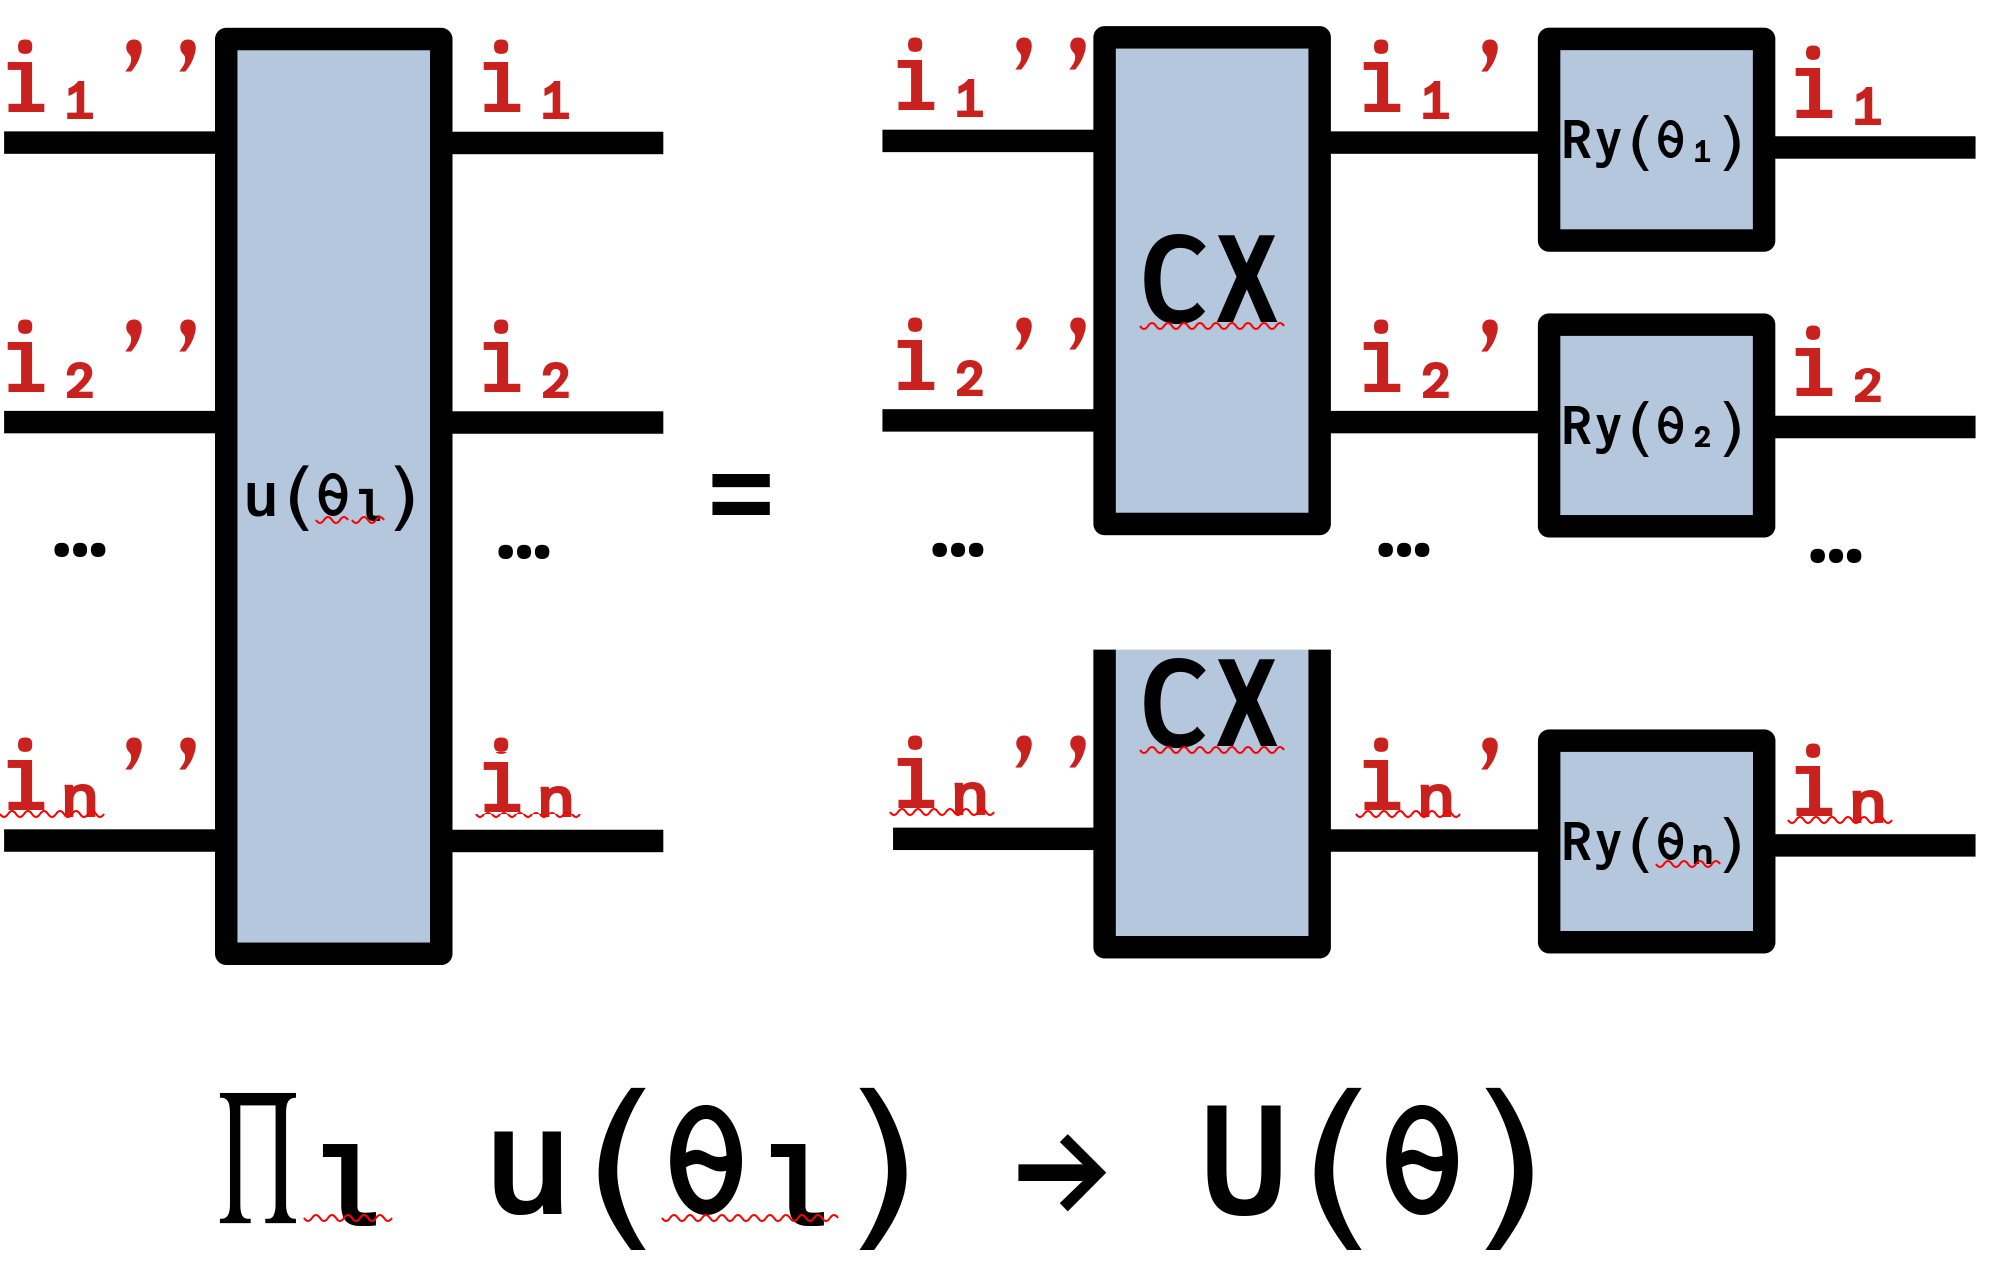
\includegraphics[width=\textwidth]{
  slides/assets/Un.png
}
\end{center}
\vspace*{0.0cm}
\end{onlyenv}

\end{column}

\end{columns}

\end{frame}
